\documentclass[12pt, fleqn, openany]{studyGuide}
\setstretch{1.4}
\enableInlineReview
\renewcommand{\VMBookTitle}{Graphical Questions Review}
\renewcommand{\VMBookSubtitle}{Grade 7 --- Bank: 2 --- Chapter: 1 --- Graphical Questions}
\renewcommand{\VMFooterURL}{https://viewmath.com/grade7}
\renewcommand{\VMFooterURLDisplay}{ViewMath.com/Grade7}
\begin{document}

\begin{center}
\begin{tcolorbox}[
	enhanced,
	colback=white,
	colframe=funTeal!60,
	boxrule=1.5pt,
	arc=10pt,
	outer arc=10pt,
	width=0.9\linewidth,
	halign=center,
	top=5mm, bottom=5mm,
]
	{\Large\bfseries\sffamily\color{funTealDark}Graphical Questions}\\[2mm]
	{\large\sffamily\color{funGrayDark}Grade 7 --- Bank: 2 --- Chapter: 1 --- Graphical Questions}\\[2mm]
	{\normalsize\sffamily\color{funGrayDark}Audit visual elements below}
\end{tcolorbox}
\end{center}

\newpage
\section*{1-1-q23 \hfill \normalsize\texttt{tests\_questions\_bank\_2/topics/ch01-01-unit-rates-with-fractions.tex}}
\begin{practiceQuestion}{1-1-q23}{gmc}
\begin{questionText}
The bar graph below shows the distance two runners covered in $\frac{1}{3}$ hour.

\begin{center}
\begin{tikzpicture}[scale=0.8]
  \draw[thick,->] (0,0) -- (0,4.5) node[above]{\small Miles};
  \draw[thick,->] (0,0) -- (5,0);
  \fill[funBlue] (0.5,0) rectangle (2,3);
  \fill[funOrange] (2.5,0) rectangle (4,2.5);
  \node[below] at (1.25,0) {\small Runner A};
  \node[below] at (3.25,0) {\small Runner B};
  \foreach \y/\lab in {1/\frac{1}{4},2/\frac{1}{2},3/\frac{3}{4},4/1}
    \draw (-0.1,\y) -- (0.1,\y) node[left=4pt] {$\lab$};
\end{tikzpicture}
\end{center}

Which runner has the faster speed in miles per hour?
\end{questionText}
\choiceA{Runner A at $2\frac{1}{4}$ mph}
\choiceB{Runner B at $1\frac{7}{8}$ mph}
\choiceC{Runner A at $\frac{1}{4}$ mph}
\choiceD{Runner B at $1\frac{1}{2}$ mph}
\correctAnswer{A}
\explanation{From the graph, Runner A covers $\frac{3}{4}$ mile and Runner B covers about $\frac{5}{8}$ mile in $\frac{1}{3}$ hour. Runner A: $\frac{3}{4} \div \frac{1}{3} = \frac{3}{4} \times 3 = \frac{9}{4} = 2\frac{1}{4}$ mph. Runner B: $\frac{5}{8} \div \frac{1}{3} = \frac{5}{8} \times 3 = \frac{15}{8} = 1\frac{7}{8}$ mph. Runner A is faster.}
\end{practiceQuestion}

\newpage
\section*{1-1-q24 \hfill \normalsize\texttt{tests\_questions\_bank\_2/topics/ch01-01-unit-rates-with-fractions.tex}}
\begin{practiceQuestion}{1-1-q24}{gmc}
\begin{questionText}
The number line below is labeled in fourths. A snail moves from $0$ to point $P$ in $\frac{2}{3}$ hour.

\begin{center}
\begin{tikzpicture}
  \draw[thick,->] (-0.5,0) -- (5.5,0);
  \foreach \x/\lab in {0/0,1/\frac{1}{4},2/\frac{1}{2},3/\frac{3}{4},4/1,5/1\frac{1}{4}}
    \draw (\x,0.15) -- (\x,-0.15) node[below]{$\lab$};
  \fill[funRed] (3,0) circle (4pt) node[above=4pt]{\small $P$};
\end{tikzpicture}
\end{center}

What is the snail's speed in units per hour?
\end{questionText}
\choiceA{$\frac{1}{2}$}
\choiceB{$\frac{3}{4}$}
\choiceC{$1\frac{1}{8}$}
\choiceD{$1\frac{1}{4}$}
\correctAnswer{C}
\explanation{Point $P$ is at $\frac{3}{4}$ on the number line. The snail's speed is $\frac{3}{4} \div \frac{2}{3} = \frac{3}{4} \times \frac{3}{2} = \frac{9}{8} = 1\frac{1}{8}$ units per hour.}
\end{practiceQuestion}

\newpage
\section*{1-1-q27 \hfill \normalsize\texttt{tests\_questions\_bank\_2/topics/ch01-01-unit-rates-with-fractions.tex}}
\begin{practiceQuestion}{1-1-q27}{gsa}
\begin{questionText}
The double number line below shows cups of sugar and batches of cookies.

\begin{center}
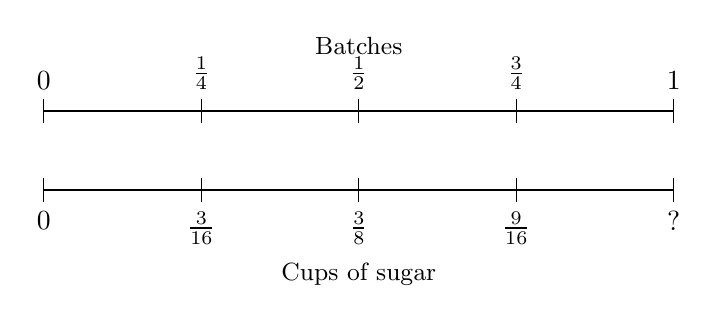
\begin{tikzpicture}[scale=1]
  \draw[thick] (0,0.5) -- (8,0.5);
  \draw[thick] (0,-0.5) -- (8,-0.5);
  \foreach \x/\lab in {0/0, 2/\frac{1}{4}, 4/\frac{1}{2}, 6/\frac{3}{4}, 8/1}
    \draw (\x,0.35) -- (\x,0.65) node[above]{$\lab$};
  \node[above] at (4,1.1) {\small Batches};
  \foreach \x/\lab in {0/0, 2/\frac{3}{16}, 4/\frac{3}{8}, 6/\frac{9}{16}, 8/?}
    \draw (\x,-0.35) -- (\x,-0.65) node[below]{$\lab$};
  \node[below] at (4,-1.3) {\small Cups of sugar};
\end{tikzpicture}
\end{center}

How many cups of sugar are needed for $1$ full batch of cookies?
\end{questionText}
\correctAnswer{$\frac{3}{4}$}
\explanation{From the double number line, $\frac{1}{4}$ batch uses $\frac{3}{16}$ cup. Find the unit rate: $\frac{3}{16} \div \frac{1}{4} = \frac{3}{16} \times 4 = \frac{12}{16} = \frac{3}{4}$ cup per batch.}
\end{practiceQuestion}

\newpage
\section*{1-2-q22 \hfill \normalsize\texttt{tests\_questions\_bank\_2/topics/ch01-02-recognizing-proportional-relationships.tex}}
\begin{practiceQuestion}{1-2-q22}{gmc}
\begin{questionText}
Look at the graph below. Does it represent a proportional relationship?

\begin{center}
\begin{tikzpicture}[scale=0.65]
  \draw[step=1,gray!20,thin] (0,0) grid (7,7);
  \draw[thick,->] (0,0) -- (7.5,0) node[right]{$x$};
  \draw[thick,->] (0,0) -- (0,7.5) node[above]{$y$};
  \foreach \x in {1,...,7} \draw (\x,0.1) -- (\x,-0.1) node[below]{\tiny \x};
  \foreach \y in {1,...,7} \draw (0.1,\y) -- (-0.1,\y) node[left]{\tiny \y};
  \draw[thick,funBlue] (0,2) -- (6,6);
  \fill[funBlue] (0,2) circle (3pt);
  \fill[funBlue] (3,4) circle (3pt);
  \fill[funBlue] (6,6) circle (3pt);
\end{tikzpicture}
\end{center}
\end{questionText}
\choiceA{Yes, because it is a straight line.}
\choiceB{Yes, because the points go up at a constant rate.}
\choiceC{No, because the line does not pass through the origin.}
\choiceD{No, because the slope is less than $1$.}
\correctAnswer{C}
\explanation{A proportional relationship must be a straight line that passes through the origin $(0, 0)$. This line crosses the $y$-axis at $(0, 2)$, so it is not proportional.}
\end{practiceQuestion}

\newpage
\section*{1-2-q24 \hfill \normalsize\texttt{tests\_questions\_bank\_2/topics/ch01-02-recognizing-proportional-relationships.tex}}
\begin{practiceQuestion}{1-2-q24}{gmc}
\begin{questionText}
Two lines are graphed on the same coordinate plane. Line $A$ passes through $(0, 0)$ and $(5, 15)$. Line $B$ passes through $(0, 4)$ and $(5, 19)$.

\begin{center}
\begin{tikzpicture}[scale=0.32]
  \draw[step=2,gray!20,thin] (0,0) grid (10,20);
  \draw[thick,->] (0,0) -- (10.5,0) node[right]{$x$};
  \draw[thick,->] (0,0) -- (0,21) node[above]{$y$};
  \foreach \x in {2,4,6,8,10} \draw (\x,0.2) -- (\x,-0.2) node[below]{\tiny \x};
  \foreach \y in {4,8,12,16,20} \draw (0.2,\y) -- (-0.2,\y) node[left]{\tiny \y};
  \draw[thick,funBlue] (0,0) -- (7,21);
  \draw[thick,funRed] (0,4) -- (6,22);
  \node[right,funBlue] at (6,18) {\small $A$};
  \node[right,funRed] at (5.5,20.5) {\small $B$};
\end{tikzpicture}
\end{center}

Which line represents a proportional relationship?
\end{questionText}
\choiceA{Only Line $A$}
\choiceB{Only Line $B$}
\choiceC{Both lines}
\choiceD{Neither line}
\correctAnswer{A}
\explanation{Line $A$ passes through the origin $(0, 0)$ and is straight, so it is proportional. Line $B$ passes through $(0, 4)$, which means it has a $y$-intercept of $4$ and is not proportional.}
\end{practiceQuestion}

\newpage
\section*{1-2-q26 \hfill \normalsize\texttt{tests\_questions\_bank\_2/topics/ch01-02-recognizing-proportional-relationships.tex}}
\begin{practiceQuestion}{1-2-q26}{gsa}
\begin{questionText}
The scatter plot below shows the heights of plants (in cm) after different numbers of weeks.

\begin{center}
\begin{tikzpicture}[scale=0.55]
  \draw[step=1,gray!20,thin] (0,0) grid (8,10);
  \draw[thick,->] (0,0) -- (8.5,0) node[right]{\small Weeks};
  \draw[thick,->] (0,0) -- (0,10.5) node[above]{\small Height (cm)};
  \foreach \x in {1,...,8} \draw (\x,0.1) -- (\x,-0.1) node[below]{\tiny \x};
  \foreach \y in {1,...,10} \draw (0.1,\y) -- (-0.1,\y) node[left]{\tiny \y};
  \fill[funGreen] (0,0) circle (4pt);
  \fill[funGreen] (2,3) circle (4pt);
  \fill[funGreen] (4,6) circle (4pt);
  \fill[funGreen] (6,9) circle (4pt);
\end{tikzpicture}
\end{center}

Is this a proportional relationship? If yes, what is the growth rate per week?
\end{questionText}
\correctAnswer{$1.5$ cm per week}
\explanation{The points $(0,0)$, $(2,3)$, $(4,6)$, and $(6,9)$ lie on a straight line through the origin. The ratio $\frac{y}{x}$ is $\frac{3}{2} = 1.5$ for every point. The relationship is proportional at $1.5$ cm per week.}
\end{practiceQuestion}

\newpage
\section*{1-2-q27 \hfill \normalsize\texttt{tests\_questions\_bank\_2/topics/ch01-02-recognizing-proportional-relationships.tex}}
\begin{practiceQuestion}{1-2-q27}{gsa}
\begin{questionText}
The graph below shows the cost of renting kayaks.

\begin{center}
\begin{tikzpicture}[scale=0.5]
  \draw[step=1,gray!20,thin] (0,0) grid (8,10);
  \draw[thick,->] (0,0) -- (8.5,0) node[right]{\small Hours};
  \draw[thick,->] (0,0) -- (0,10.5) node[above]{\small Cost (\$)};
  \foreach \x in {1,...,8} \draw (\x,0.1) -- (\x,-0.1) node[below]{\tiny \x};
  \foreach \y in {2,4,...,10} \draw (0.1,\y) -- (-0.1,\y) node[left]{\tiny \y0};
  \fill[funPurple] (0,2) circle (4pt);
  \fill[funPurple] (1,3.5) circle (4pt);
  \fill[funPurple] (2,5) circle (4pt);
  \fill[funPurple] (4,8) circle (4pt);
  \draw[thick,funPurple] (0,2) -- (4,8);
\end{tikzpicture}
\end{center}

The $y$-axis values are in tens of dollars ($20, 40, \ldots$). Why is this relationship \textbf{not} proportional? State the reason.
\end{questionText}
\correctAnswer{The line does not pass through the origin}
\explanation{The graph starts at $(0, 20)$, meaning there is a $\$20$ base fee even for $0$ hours. A proportional relationship must pass through $(0, 0)$. Since the line starts above the origin, the relationship is not proportional.}
\end{practiceQuestion}

\newpage
\section*{1-3-q22 \hfill \normalsize\texttt{tests\_questions\_bank\_2/topics/ch01-03-finding-the-constant-of-proportionality.tex}}
\begin{practiceQuestion}{1-3-q22}{gmc}
\begin{questionText}
The graph below shows a proportional relationship. What is the constant of proportionality?

\begin{center}
\begin{tikzpicture}[scale=0.55]
  \draw[step=1,gray!20,thin] (0,0) grid (8,8);
  \draw[thick,->] (0,0) -- (8.5,0) node[right]{$x$};
  \draw[thick,->] (0,0) -- (0,8.5) node[above]{$y$};
  \foreach \x in {1,...,8} \draw (\x,0.1) -- (\x,-0.1) node[below]{\tiny \x};
  \foreach \y in {1,...,8} \draw (0.1,\y) -- (-0.1,\y) node[left]{\tiny \y};
  \draw[thick,funBlue] (0,0) -- (8,6);
  \fill[funBlue] (0,0) circle (3pt);
  \fill[funBlue] (4,3) circle (3pt);
  \fill[funBlue] (8,6) circle (3pt);
\end{tikzpicture}
\end{center}
\end{questionText}
\choiceA{$k = \frac{4}{3}$}
\choiceB{$k = \frac{3}{4}$}
\choiceC{$k = 3$}
\choiceD{$k = 4$}
\correctAnswer{B}
\explanation{Read the point $(4, 3)$ from the graph. The constant of proportionality is $k = \frac{y}{x} = \frac{3}{4}$. Check with $(8,6)$: $\frac{6}{8} = \frac{3}{4}$ \checkmark.}
\end{practiceQuestion}

\newpage
\section*{1-3-q24 \hfill \normalsize\texttt{tests\_questions\_bank\_2/topics/ch01-03-finding-the-constant-of-proportionality.tex}}
\begin{practiceQuestion}{1-3-q24}{gmc}
\begin{questionText}
Two proportional lines are graphed on the same axes. Line $P$ passes through $(3, 6)$ and Line $Q$ passes through $(3, 9)$. Both pass through the origin.

\begin{center}
\begin{tikzpicture}[scale=0.45]
  \draw[step=1,gray!20,thin] (0,0) grid (6,12);
  \draw[thick,->] (0,0) -- (6.5,0) node[right]{$x$};
  \draw[thick,->] (0,0) -- (0,12.5) node[above]{$y$};
  \foreach \x in {1,...,6} \draw (\x,0.1) -- (\x,-0.1) node[below]{\tiny \x};
  \foreach \y in {2,4,...,12} \draw (0.1,\y) -- (-0.1,\y) node[left]{\tiny \y};
  \draw[thick,funBlue] (0,0) -- (6,12);
  \draw[thick,funOrange] (0,0) -- (6,12);
  \draw[thick,funBlue] (0,0) -- (5,10);
  \draw[thick,funOrange] (0,0) -- (4,12);
  \fill[funBlue] (3,6) circle (3pt) node[right]{\tiny $P$};
  \fill[funOrange] (3,9) circle (3pt) node[left]{\tiny $Q$};
\end{tikzpicture}
\end{center}

How much greater is $k_Q$ than $k_P$?
\end{questionText}
\choiceA{$1$}
\choiceB{$3$}
\choiceC{$\frac{1}{3}$}
\choiceD{$\frac{3}{2}$}
\correctAnswer{A}
\explanation{$k_P = \frac{6}{3} = 2$ and $k_Q = \frac{9}{3} = 3$. The difference is $3 - 2 = 1$.}
\end{practiceQuestion}

\newpage
\section*{1-3-q25 \hfill \normalsize\texttt{tests\_questions\_bank\_2/topics/ch01-03-finding-the-constant-of-proportionality.tex}}
\begin{practiceQuestion}{1-3-q25}{gsa}
\begin{questionText}
The graph below shows the cost of renting roller skates per hour.

\begin{center}
\begin{tikzpicture}[scale=0.5]
  \draw[step=1,gray!20,thin] (0,0) grid (8,10);
  \draw[thick,->] (0,0) -- (8.5,0) node[right]{\small Hours};
  \draw[thick,->] (0,0) -- (0,10.5) node[above]{\small Cost (\$)};
  \foreach \x in {1,...,8} \draw (\x,0.1) -- (\x,-0.1) node[below]{\tiny \x};
  \foreach \y in {1,...,10} \draw (0.1,\y) -- (-0.1,\y) node[left]{\tiny \y};
  \draw[thick,funGreen] (0,0) -- (8,10);
  \fill[funGreen] (0,0) circle (3pt);
  \fill[funGreen] (2,2.5) circle (3pt);
  \fill[funGreen] (4,5) circle (3pt);
  \fill[funGreen] (8,10) circle (3pt);
\end{tikzpicture}
\end{center}

What is the constant of proportionality? Include units.
\end{questionText}
\correctAnswer{$\$1.25$ per hour}
\explanation{Use the point $(4, 5)$: $k = \frac{5}{4} = 1.25$ dollars per hour. Check: $\frac{2.5}{2} = 1.25$ and $\frac{10}{8} = 1.25$ \checkmark.}
\end{practiceQuestion}

\newpage
\section*{1-3-q26 \hfill \normalsize\texttt{tests\_questions\_bank\_2/topics/ch01-03-finding-the-constant-of-proportionality.tex}}
\begin{practiceQuestion}{1-3-q26}{gsa}
\begin{questionText}
The double number line below shows a proportional relationship between feet and seconds.

\begin{center}
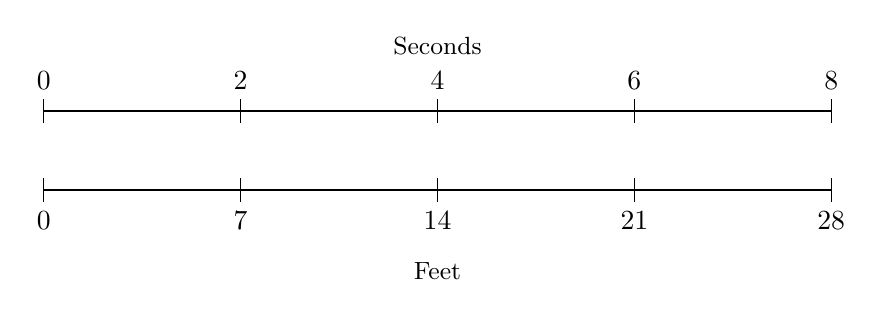
\begin{tikzpicture}[scale=1]
  \draw[thick] (0,0.5) -- (10,0.5);
  \draw[thick] (0,-0.5) -- (10,-0.5);
  \foreach \x/\lab in {0/0, 2.5/2, 5/4, 7.5/6, 10/8}
    \draw (\x,0.35) -- (\x,0.65) node[above]{$\lab$};
  \node[above] at (5,1.1) {\small Seconds};
  \foreach \x/\lab in {0/0, 2.5/7, 5/14, 7.5/21, 10/28}
    \draw (\x,-0.35) -- (\x,-0.65) node[below]{$\lab$};
  \node[below] at (5,-1.3) {\small Feet};
\end{tikzpicture}
\end{center}

What is the constant of proportionality in feet per second?
\end{questionText}
\correctAnswer{$3.5$}
\explanation{Divide feet by seconds from any pair: $\frac{7}{2} = 3.5$, $\frac{14}{4} = 3.5$, $\frac{21}{6} = 3.5$, $\frac{28}{8} = 3.5$. The constant is $3.5$ feet per second.}
\end{practiceQuestion}

\newpage
\section*{1-4-q22 \hfill \normalsize\texttt{tests\_questions\_bank\_2/topics/ch01-04-writing-equations-for-proportional-relationships.tex}}
\begin{practiceQuestion}{1-4-q22}{gmc}
\begin{questionText}
The graph below shows a proportional relationship between hours worked and money earned.

\begin{center}
\begin{tikzpicture}[scale=0.5]
  \draw[step=1,gray!20,thin] (0,0) grid (8,10);
  \draw[thick,->] (0,0) -- (8.5,0) node[right]{\small Hours};
  \draw[thick,->] (0,0) -- (0,10.5) node[above]{\small Earnings (\$)};
  \foreach \x in {1,...,8} \draw (\x,0.1) -- (\x,-0.1) node[below]{\tiny \x};
  \foreach \y in {1,...,10} \draw (0.1,\y) -- (-0.1,\y) node[left]{\tiny \y};
  \draw[thick,funBlue] (0,0) -- (8,10);
  \fill[funBlue] (0,0) circle (3pt);
  \fill[funBlue] (4,5) circle (3pt);
  \fill[funBlue] (8,10) circle (3pt);
\end{tikzpicture}
\end{center}

Which equation represents this graph?
\end{questionText}
\choiceA{$e = 0.8h$}
\choiceB{$e = 1.25h$}
\choiceC{$e = 5h$}
\choiceD{$e = 2h$}
\correctAnswer{B}
\explanation{From the graph, the point $(4, 5)$ gives $k = \frac{5}{4} = 1.25$. The equation is $e = 1.25h$.}
\end{practiceQuestion}

\newpage
\section*{1-4-q24 \hfill \normalsize\texttt{tests\_questions\_bank\_2/topics/ch01-04-writing-equations-for-proportional-relationships.tex}}
\begin{practiceQuestion}{1-4-q24}{gmc}
\begin{questionText}
The double number line below shows the proportional relationship between liters of paint and square meters covered.

\begin{center}
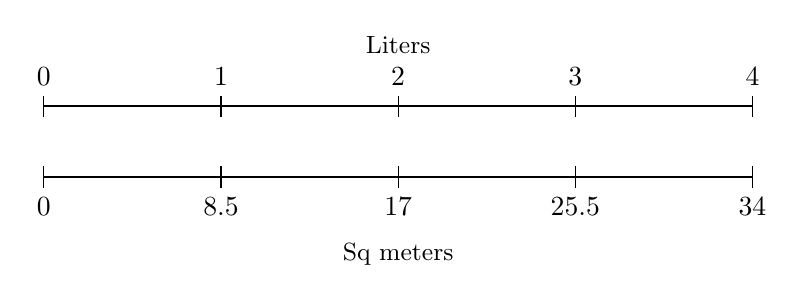
\begin{tikzpicture}[scale=0.9]
  \draw[thick] (0,0.5) -- (10,0.5);
  \draw[thick] (0,-0.5) -- (10,-0.5);
  \foreach \x/\lab in {0/0, 2.5/1, 5/2, 7.5/3, 10/4}
    \draw (\x,0.35) -- (\x,0.65) node[above]{$\lab$};
  \node[above] at (5,1.1) {\small Liters};
  \foreach \x/\lab in {0/0, 2.5/8.5, 5/17, 7.5/25.5, 10/34}
    \draw (\x,-0.35) -- (\x,-0.65) node[below]{$\lab$};
  \node[below] at (5,-1.3) {\small Sq meters};
\end{tikzpicture}
\end{center}

Which equation represents the relationship?
\end{questionText}
\choiceA{$s = 8.5l$}
\choiceB{$l = 8.5s$}
\choiceC{$s = l + 8.5$}
\choiceD{$s = 4.25l$}
\correctAnswer{A}
\explanation{From the double number line, $1$ liter covers $8.5$ sq meters. The equation is $s = 8.5l$. Check: $2$ liters covers $8.5 \times 2 = 17$ \checkmark.}
\end{practiceQuestion}

\newpage
\section*{1-4-q25 \hfill \normalsize\texttt{tests\_questions\_bank\_2/topics/ch01-04-writing-equations-for-proportional-relationships.tex}}
\begin{practiceQuestion}{1-4-q25}{gsa}
\begin{questionText}
The graph below shows a proportional relationship.

\begin{center}
\begin{tikzpicture}[scale=0.5]
  \draw[step=1,gray!20,thin] (0,0) grid (10,8);
  \draw[thick,->] (0,0) -- (10.5,0) node[right]{$x$};
  \draw[thick,->] (0,0) -- (0,8.5) node[above]{$y$};
  \foreach \x in {2,4,...,10} \draw (\x,0.1) -- (\x,-0.1) node[below]{\tiny \x};
  \foreach \y in {1,...,8} \draw (0.1,\y) -- (-0.1,\y) node[left]{\tiny \y};
  \draw[thick,funOrange] (0,0) -- (10,6);
  \fill[funOrange] (0,0) circle (3pt);
  \fill[funOrange] (5,3) circle (3pt);
  \fill[funOrange] (10,6) circle (3pt);
\end{tikzpicture}
\end{center}

Write the equation for this proportional relationship.
\end{questionText}
\correctAnswer{$y = 0.6x$}
\explanation{From the graph, the point $(5, 3)$ gives $k = \frac{3}{5} = 0.6$. The equation is $y = 0.6x$. Check: $0.6 \times 10 = 6$ \checkmark.}
\end{practiceQuestion}

\newpage
\section*{1-4-q27 \hfill \normalsize\texttt{tests\_questions\_bank\_2/topics/ch01-04-writing-equations-for-proportional-relationships.tex}}
\begin{practiceQuestion}{1-4-q27}{gsa}
\begin{questionText}
A proportional graph passes through the points shown below.

\begin{center}
\begin{tikzpicture}[scale=0.45]
  \draw[step=1,gray!20,thin] (0,0) grid (10,10);
  \draw[thick,->] (0,0) -- (10.5,0) node[right]{$x$};
  \draw[thick,->] (0,0) -- (0,10.5) node[above]{$y$};
  \foreach \x in {1,...,10} \draw (\x,0.1) -- (\x,-0.1) node[below]{\tiny \x};
  \foreach \y in {1,...,10} \draw (0.1,\y) -- (-0.1,\y) node[left]{\tiny \y};
  \draw[thick,funPurple] (0,0) -- (10,7.5);
  \fill[funPurple] (0,0) circle (3pt);
  \fill[funPurple] (4,3) circle (3pt);
  \fill[funPurple] (8,6) circle (3pt);
\end{tikzpicture}
\end{center}

Write the equation, and find the value of $y$ when $x = 14$.
\end{questionText}
\correctAnswer{$10.5$}
\explanation{From the point $(4, 3)$: $k = \frac{3}{4} = 0.75$. The equation is $y = 0.75x$. Substitute $x = 14$: $y = 0.75 \times 14 = 10.5$.}
\end{practiceQuestion}

\newpage
\section*{1-5-q22 \hfill \normalsize\texttt{tests\_questions\_bank\_2/topics/ch01-05-graphing-proportional-relationships.tex}}
\begin{practiceQuestion}{1-5-q22}{gmc}
\begin{questionText}
The graph below shows the distance a train travels over time.

\begin{center}
\begin{tikzpicture}[scale=0.5]
  \draw[step=1,gray!20,thin] (0,0) grid (8,10);
  \draw[thick,->] (0,0) -- (8.5,0) node[right]{\small Hours};
  \draw[thick,->] (0,0) -- (0,10.5) node[above]{\small Distance (mi)};
  \foreach \x in {1,...,8} \draw (\x,0.1) -- (\x,-0.1) node[below]{\tiny \x};
  \foreach \y/\lab in {1/50,2/100,3/150,4/200,5/250,6/300,7/350,8/400,9/450,10/500}
    \draw (0.1,\y) -- (-0.1,\y) node[left]{\tiny \lab};
  \draw[thick,funBlue] (0,0) -- (8,6.4);
  \fill[funBlue] (0,0) circle (3pt);
  \fill[funBlue] (1,0.8) circle (3pt);
  \fill[funBlue] (5,4) circle (3pt);
\end{tikzpicture}
\end{center}

What is the train's speed in miles per hour?
\end{questionText}
\choiceA{$40$ mph}
\choiceB{$50$ mph}
\choiceC{$80$ mph}
\choiceD{$100$ mph}
\correctAnswer{A}
\explanation{From the point $(1, 0.8)$ on the graph, and since each grid unit on the $y$-axis equals $50$ miles, the $y$-value at $x = 1$ is $0.8 \times 50 = 40$ miles. The unit rate from the point $(5, 200)$ confirms: $200 \div 5 = 40$ mph.}
\end{practiceQuestion}

\newpage
\section*{1-5-q23 \hfill \normalsize\texttt{tests\_questions\_bank\_2/topics/ch01-05-graphing-proportional-relationships.tex}}
\begin{practiceQuestion}{1-5-q23}{gmc}
\begin{questionText}
Two proportional lines are graphed below. Line $A$ (blue) passes through $(4, 6)$. Line $B$ (orange) passes through $(4, 10)$.

\begin{center}
\begin{tikzpicture}[scale=0.5]
  \draw[step=1,gray!20,thin] (0,0) grid (8,12);
  \draw[thick,->] (0,0) -- (8.5,0) node[right]{$x$};
  \draw[thick,->] (0,0) -- (0,12.5) node[above]{$y$};
  \foreach \x in {1,...,8} \draw (\x,0.1) -- (\x,-0.1) node[below]{\tiny \x};
  \foreach \y in {2,4,...,12} \draw (0.1,\y) -- (-0.1,\y) node[left]{\tiny \y};
  \draw[thick,funBlue] (0,0) -- (8,12);
  \draw[thick,funOrange] (0,0) -- (5,12.5);
  \fill[funBlue] (4,6) circle (3pt) node[right=2pt]{\tiny $A$};
  \fill[funOrange] (4,10) circle (3pt) node[left=2pt]{\tiny $B$};
\end{tikzpicture}
\end{center}

What is the unit rate of Line $B$?
\end{questionText}
\choiceA{$1.5$}
\choiceB{$2$}
\choiceC{$2.5$}
\choiceD{$4$}
\correctAnswer{C}
\explanation{Line $B$ passes through $(4, 10)$ and the origin: $k = \frac{10}{4} = 2.5$. The unit rate is $2.5$.}
\end{practiceQuestion}

\newpage
\section*{1-5-q24 \hfill \normalsize\texttt{tests\_questions\_bank\_2/topics/ch01-05-graphing-proportional-relationships.tex}}
\begin{practiceQuestion}{1-5-q24}{gmc}
\begin{questionText}
The graph below represents a proportional relationship between cups of flour and number of cakes baked.

\begin{center}
\begin{tikzpicture}[scale=0.5]
  \draw[step=1,gray!20,thin] (0,0) grid (10,8);
  \draw[thick,->] (0,0) -- (10.5,0) node[right]{\small Cakes};
  \draw[thick,->] (0,0) -- (0,8.5) node[above]{\small Cups of flour};
  \foreach \x in {1,...,10} \draw (\x,0.1) -- (\x,-0.1) node[below]{\tiny \x};
  \foreach \y in {1,...,8} \draw (0.1,\y) -- (-0.1,\y) node[left]{\tiny \y};
  \draw[thick,funGreen] (0,0) -- (10,7.5);
  \fill[funGreen] (0,0) circle (3pt);
  \fill[funGreen] (4,3) circle (3pt);
  \fill[funGreen] (8,6) circle (3pt);
\end{tikzpicture}
\end{center}

How many cups of flour are needed for $12$ cakes?
\end{questionText}
\choiceA{$6$}
\choiceB{$8$}
\choiceC{$9$}
\choiceD{$12$}
\correctAnswer{C}
\explanation{From the point $(4, 3)$: $k = \frac{3}{4} = 0.75$ cups per cake. For $12$ cakes: $0.75 \times 12 = 9$ cups.}
\end{practiceQuestion}

\newpage
\section*{1-5-q25 \hfill \normalsize\texttt{tests\_questions\_bank\_2/topics/ch01-05-graphing-proportional-relationships.tex}}
\begin{practiceQuestion}{1-5-q25}{gsa}
\begin{questionText}
The graph below shows two proportional lines.

\begin{center}
\begin{tikzpicture}[scale=0.5]
  \draw[step=1,gray!20,thin] (0,0) grid (8,10);
  \draw[thick,->] (0,0) -- (8.5,0) node[right]{$x$};
  \draw[thick,->] (0,0) -- (0,10.5) node[above]{$y$};
  \foreach \x in {1,...,8} \draw (\x,0.1) -- (\x,-0.1) node[below]{\tiny \x};
  \foreach \y in {1,...,10} \draw (0.1,\y) -- (-0.1,\y) node[left]{\tiny \y};
  \draw[thick,funBlue] (0,0) -- (8,8);
  \draw[thick,funRed] (0,0) -- (5,10);
  \fill[funBlue] (4,4) circle (3pt) node[below right]{\tiny $A(4,4)$};
  \fill[funRed] (5,10) circle (3pt) node[left]{\tiny $B(5,10)$};
\end{tikzpicture}
\end{center}

What is the difference in the unit rates of Line $B$ and Line $A$?
\end{questionText}
\correctAnswer{$1$}
\explanation{Line $A$: $k = \frac{4}{4} = 1$. Line $B$: $k = \frac{10}{5} = 2$. Difference: $2 - 1 = 1$.}
\end{practiceQuestion}

\newpage
\section*{1-5-q26 \hfill \normalsize\texttt{tests\_questions\_bank\_2/topics/ch01-05-graphing-proportional-relationships.tex}}
\begin{practiceQuestion}{1-5-q26}{gsa}
\begin{questionText}
The coordinate plane below shows a proportional relationship between time (seconds) and distance (meters).

\begin{center}
\begin{tikzpicture}[scale=0.55]
  \draw[step=1,gray!20,thin] (0,0) grid (8,10);
  \draw[thick,->] (0,0) -- (8.5,0) node[right]{\small Seconds};
  \draw[thick,->] (0,0) -- (0,10.5) node[above]{\small Meters};
  \foreach \x in {1,...,8} \draw (\x,0.1) -- (\x,-0.1) node[below]{\tiny \x};
  \foreach \y in {1,...,10} \draw (0.1,\y) -- (-0.1,\y) node[left]{\tiny \y};
  \draw[thick,funOrange] (0,0) -- (8,7);
  \fill[funOrange] (0,0) circle (3pt);
  \fill[funOrange] (4,3.5) circle (3pt);
  \fill[funOrange] (8,7) circle (3pt);
\end{tikzpicture}
\end{center}

What is the speed in meters per second? How far does the object travel in $12$ seconds?
\end{questionText}
\correctAnswer{$10.5$ meters}
\explanation{From $(8, 7)$: $k = \frac{7}{8} = 0.875$ m/s. For $12$ seconds: $0.875 \times 12 = 10.5$ meters.}
\end{practiceQuestion}

\newpage
\section*{1-5-q27 \hfill \normalsize\texttt{tests\_questions\_bank\_2/topics/ch01-05-graphing-proportional-relationships.tex}}
\begin{practiceQuestion}{1-5-q27}{gsa}
\begin{questionText}
The graph below shows two workers' earnings over time. Both pass through the origin.

\begin{center}
\begin{tikzpicture}[scale=0.5]
  \draw[step=1,gray!20,thin] (0,0) grid (8,10);
  \draw[thick,->] (0,0) -- (8.5,0) node[right]{\small Hours};
  \draw[thick,->] (0,0) -- (0,10.5) node[above]{\small Earnings (\$)};
  \foreach \x in {1,...,8} \draw (\x,0.1) -- (\x,-0.1) node[below]{\tiny \x};
  \foreach \y/\lab in {2/20,4/40,6/60,8/80,10/100}
    \draw (0.1,\y) -- (-0.1,\y) node[left]{\tiny \lab};
  \draw[thick,funBlue] (0,0) -- (8,9.6);
  \draw[thick,funRed] (0,0) -- (8,6.4);
  \fill[funBlue] (5,6) circle (3pt) node[above left]{\tiny Worker $A$};
  \fill[funRed] (5,4) circle (3pt) node[below right]{\tiny Worker $B$};
\end{tikzpicture}
\end{center}

Each $y$-axis unit equals $\$10$. How much more does Worker $A$ earn than Worker $B$ in an $8$-hour shift?
\end{questionText}
\correctAnswer{$\$32$}
\explanation{Each $y$-unit is $\$10$, so Worker $A$ at $(5, 6)$ earns $\$60$ in $5$ hours ($\$12$/hr) and Worker $B$ at $(5, 4)$ earns $\$40$ in $5$ hours ($\$8$/hr). In $8$ hours: $A$ earns $12 \times 8 = \$96$ and $B$ earns $8 \times 8 = \$64$. Difference: $96 - 64 = \$32$.}
\end{practiceQuestion}

\newpage
\section*{1-6-q23 \hfill \normalsize\texttt{tests\_questions\_bank\_2/topics/ch01-06-applying-proportional-reasoning.tex}}
\begin{practiceQuestion}{1-6-q23}{gmc}
\begin{questionText}
The bar graph below shows the cost per pound of two different cheeses.

\begin{center}
\begin{tikzpicture}[scale=0.7]
  \draw[thick,->] (0,0) -- (0,5) node[above]{\small \$/lb};
  \draw[thick,->] (0,0) -- (5.5,0);
  \fill[funBlue] (0.5,0) rectangle (2,3.6);
  \fill[funOrange] (2.5,0) rectangle (4,4.5);
  \node[below] at (1.25,-0.1) {\small Cheddar};
  \node[below] at (3.25,-0.1) {\small Swiss};
  \foreach \y/\lab in {1/\$2,2/\$4,3/\$6,4/\$8}
    \draw (-0.1,\y) -- (0.1,\y) node[left=4pt]{\small \lab};
\end{tikzpicture}
\end{center}

Marco buys $3$ pounds of cheddar and $2$ pounds of Swiss. Each bar unit equals $\$2$. What is the total cost?
\end{questionText}
\choiceA{$\$28.80$}
\choiceB{$\$30.60$}
\choiceC{$\$36.00$}
\choiceD{$\$39.60$}
\correctAnswer{D}
\explanation{Each grid unit on the y-axis is $\$2$. Cheddar bar reaches $3.6$ units $= 3.6 \times 2 = \$7.20$/lb. Swiss bar reaches $4.5$ units $= 4.5 \times 2 = \$9.00$/lb. Cheddar: $7.20 \times 3 = \$21.60$. Swiss: $9.00 \times 2 = \$18.00$. Total: $21.60 + 18.00 = \$39.60$.}
\end{practiceQuestion}

\newpage
\section*{1-6-q24 \hfill \normalsize\texttt{tests\_questions\_bank\_2/topics/ch01-06-applying-proportional-reasoning.tex}}
\begin{practiceQuestion}{1-6-q24}{gmc}
\begin{questionText}
A map uses the scale shown below.

\begin{center}
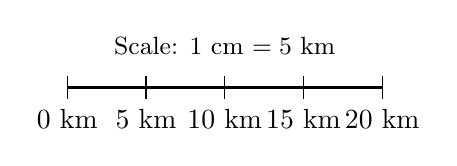
\begin{tikzpicture}
  \draw[thick] (0,0) -- (4,0);
  \foreach \x/\lab in {0/0,1/5,2/10,3/15,4/20}
    \draw (\x,0.15) -- (\x,-0.15) node[below]{$\lab$ km};
  \node[above] at (2,0.3) {\small Scale: $1$ cm $= 5$ km};
\end{tikzpicture}
\end{center}

On the map, a road is $7.4$ cm long. What is the actual distance?
\end{questionText}
\choiceA{$12.4$ km}
\choiceB{$37$ km}
\choiceC{$42$ km}
\choiceD{$74$ km}
\correctAnswer{B}
\explanation{Each centimeter on the map equals $5$ km. Multiply: $7.4 \times 5 = 37$ km.}
\end{practiceQuestion}

\newpage
\section*{1-6-q26 \hfill \normalsize\texttt{tests\_questions\_bank\_2/topics/ch01-06-applying-proportional-reasoning.tex}}
\begin{practiceQuestion}{1-6-q26}{gsa}
\begin{questionText}
The double number line shows the relationship between ounces of dog food and the number of dogs fed.

\begin{center}
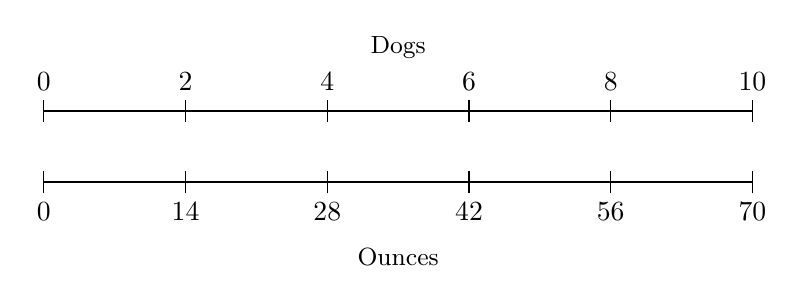
\begin{tikzpicture}[scale=0.9]
  \draw[thick] (0,0.5) -- (10,0.5);
  \draw[thick] (0,-0.5) -- (10,-0.5);
  \foreach \x/\lab in {0/0, 2/2, 4/4, 6/6, 8/8, 10/10}
    \draw (\x,0.35) -- (\x,0.65) node[above]{$\lab$};
  \node[above] at (5,1.1) {\small Dogs};
  \foreach \x/\lab in {0/0, 2/14, 4/28, 6/42, 8/56, 10/70}
    \draw (\x,-0.35) -- (\x,-0.65) node[below]{$\lab$};
  \node[below] at (5,-1.3) {\small Ounces};
\end{tikzpicture}
\end{center}

How many ounces of dog food are needed for $15$ dogs?
\end{questionText}
\correctAnswer{$105$}
\explanation{From the double number line, each dog needs $\frac{14}{2} = 7$ ounces. For $15$ dogs: $7 \times 15 = 105$ ounces.}
\end{practiceQuestion}

\newpage
\section*{1-6-q27 \hfill \normalsize\texttt{tests\_questions\_bank\_2/topics/ch01-06-applying-proportional-reasoning.tex}}
\begin{practiceQuestion}{1-6-q27}{gsa}
\begin{questionText}
The graph below shows the proportional relationship between hours and the number of bracelets a crafter makes.

\begin{center}
\begin{tikzpicture}[scale=0.5]
  \draw[step=1,gray!20,thin] (0,0) grid (8,10);
  \draw[thick,->] (0,0) -- (8.5,0) node[right]{\small Hours};
  \draw[thick,->] (0,0) -- (0,10.5) node[above]{\small Bracelets};
  \foreach \x in {1,...,8} \draw (\x,0.1) -- (\x,-0.1) node[below]{\tiny \x};
  \foreach \y in {1,...,10} \draw (0.1,\y) -- (-0.1,\y) node[left]{\tiny \y};
  \draw[thick,funPurple] (0,0) -- (8,6);
  \fill[funPurple] (0,0) circle (3pt);
  \fill[funPurple] (4,3) circle (3pt);
  \fill[funPurple] (8,6) circle (3pt);
\end{tikzpicture}
\end{center}

How many bracelets can the crafter make in a $10$-hour day?
\end{questionText}
\correctAnswer{$7.5$}
\explanation{From the point $(4, 3)$: $k = \frac{3}{4} = 0.75$ bracelets per hour. For $10$ hours: $0.75 \times 10 = 7.5$ bracelets.}
\end{practiceQuestion}

\newpage
\section*{m-1-6-q23 \hfill \normalsize\texttt{tests\_questions\_bank\_2/topics\_modified/ch01-06-applying-proportional-reasoning.tex}}
\begin{practiceQuestion}{m-1-6-q23}{gmc}
\begin{questionText}
The graph below shows two workers' earnings over time.

\begin{center}
\begin{tikzpicture}[scale=0.5]
  \draw[step=1,gray!20,thin] (0,0) grid (10,10);
  \draw[thick,->] (0,0) -- (10.5,0) node[right]{\small Hours};
  \draw[thick,->] (0,0) -- (0,10.5) node[above]{\small Earnings (\$)};
  \foreach \x in {1,...,10} \draw (\x,0.1) -- (\x,-0.1) node[below]{\tiny \x};
  \foreach \y/\lab in {2/20,4/40,6/60,8/80,10/100}
    \draw (0.1,\y) -- (-0.1,\y) node[left]{\tiny \lab};
  \draw[thick,funBlue] (0,0) -- (10,9);
  \draw[thick,funRed] (0,0) -- (10,6);
  \fill[funBlue] (0,0) circle (3pt); \fill[funBlue] (10,9) circle (3pt);
  \fill[funRed] (0,0) circle (3pt); \fill[funRed] (10,6) circle (3pt);
  \node[funBlue,right] at (10,9) {\tiny Worker A};
  \node[funRed,right] at (10,6) {\tiny Worker B};
\end{tikzpicture}
\end{center}

Each y-axis unit $= \$10$. Which is the best estimate of the combined earnings after $6$ hours?
\end{questionText}
\choiceA{About $\$60$}
\choiceB{About $\$72$}
\choiceC{About $\$90$}
\choiceD{About $\$108$}
\correctAnswer{C}
\explanation{Worker A: slope $= \frac{90}{10} = \$9$/hr. At $6$ hrs: $9 \times 6 = \$54$. Worker B: slope $= \frac{60}{10} = \$6$/hr. At $6$ hrs: $6 \times 6 = \$36$. Combined: $54 + 36 = \$90$.}
\end{practiceQuestion}

\newpage
\section*{m-1-6-q24 \hfill \normalsize\texttt{tests\_questions\_bank\_2/topics\_modified/ch01-06-applying-proportional-reasoning.tex}}
\begin{practiceQuestion}{m-1-6-q24}{gmc}
\begin{questionText}
A double number line shows the relationship between gallons of paint and square feet of wall covered.

\begin{center}
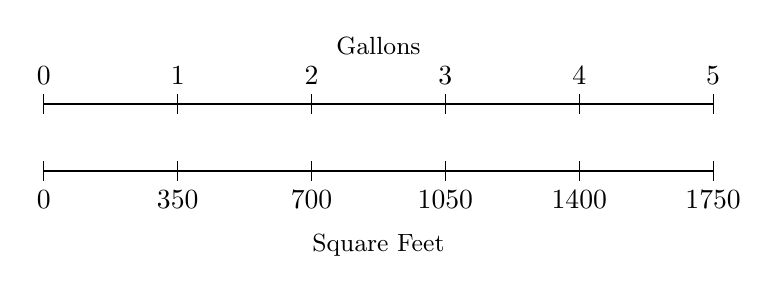
\begin{tikzpicture}[scale=0.85]
  \draw[thick] (0,0.5) -- (10,0.5);
  \draw[thick] (0,-0.5) -- (10,-0.5);
  \foreach \x/\lab in {0/0, 2/1, 4/2, 6/3, 8/4, 10/5}
    \draw (\x,0.35) -- (\x,0.65) node[above]{$\lab$};
  \node[above] at (5,1.1) {\small Gallons};
  \foreach \x/\lab in {0/0, 2/350, 4/700, 6/1050, 8/1400, 10/1750}
    \draw (\x,-0.35) -- (\x,-0.65) node[below]{$\lab$};
  \node[below] at (5,-1.3) {\small Square Feet};
\end{tikzpicture}
\end{center}

A room has $2{,}100$ sq ft of wall. Estimate the number of gallons needed.
\end{questionText}
\choiceA{$5$}
\choiceB{$6$}
\choiceC{$7$}
\choiceD{$8$}
\correctAnswer{B}
\explanation{Rate: $350$ sq ft per gallon. Gallons: $2{,}100 \div 350 = 6$.}
\end{practiceQuestion}

\newpage
\section*{m-1-6-q26 \hfill \normalsize\texttt{tests\_questions\_bank\_2/topics\_modified/ch01-06-applying-proportional-reasoning.tex}}
\begin{practiceQuestion}{m-1-6-q26}{gsa}
\begin{questionText}
The graph below shows two streaming services' monthly data usage.

\begin{center}
\begin{tikzpicture}[scale=0.5]
  \draw[step=1,gray!20,thin] (0,0) grid (8,10);
  \draw[thick,->] (0,0) -- (8.5,0) node[right]{\small Hours};
  \draw[thick,->] (0,0) -- (0,10.5) node[above]{\small GB};
  \foreach \x in {1,...,8} \draw (\x,0.1) -- (\x,-0.1) node[below]{\tiny \x};
  \foreach \y in {2,4,6,8,10} \draw (0.1,\y) -- (-0.1,\y) node[left]{\tiny \y};
  \draw[thick,funGreen] (0,0) -- (8,6);
  \draw[thick,funOrange] (0,0) -- (8,4);
  \fill[funGreen] (4,3) circle (3pt);
  \fill[funOrange] (4,2) circle (3pt);
  \node[funGreen,right] at (8.1,6) {\tiny Service A};
  \node[funOrange,right] at (8.1,4) {\tiny Service B};
\end{tikzpicture}
\end{center}

How many more GB does Service A use than Service B in $12$ hours?
\end{questionText}
\correctAnswer{$3$ GB}
\explanation{Service A: from $(4, 3)$, rate $= \frac{3}{4} = 0.75$ GB/hr. In $12$ hrs: $0.75 \times 12 = 9$ GB. Service B: from $(4, 2)$, rate $= \frac{2}{4} = 0.5$ GB/hr. In $12$ hrs: $0.5 \times 12 = 6$ GB. Difference: $9 - 6 = 3$ GB.}
\end{practiceQuestion}

\newpage
\section*{1-7-q22 \hfill \normalsize\texttt{tests\_questions\_bank\_2/topics\_additional/ch01-07-proportional-reasoning-with-scale-models.tex}}
\begin{practiceQuestion}{1-7-q22}{gmc}
\begin{questionText}
The scale drawing below shows the floor plan of a rectangular room.

\begin{center}
\begin{tikzpicture}[scale=0.9]
  \draw[thick,funBlue,fill=funBlue!10] (0,0) rectangle (5,3);
  \draw[<->,thick] (0,-0.4) -- (5,-0.4) node[midway,below]{\small $10$ cm};
  \draw[<->,thick] (-0.4,0) -- (-0.4,3) node[midway,left]{\small $6$ cm};
  \node at (2.5,1.5) {\small Room};
  \node at (2.5,-1.2) {\small Scale: $1$ cm $= 2$ ft};
\end{tikzpicture}
\end{center}

What is the actual area of the room?
\end{questionText}
\choiceA{$60$ sq ft}
\choiceB{$120$ sq ft}
\choiceC{$200$ sq ft}
\choiceD{$240$ sq ft}
\correctAnswer{D}
\explanation{Actual length $= 10 \times 2 = 20$ ft. Actual width $= 6 \times 2 = 12$ ft. Area $= 20 \times 12 = 240$ sq ft.}
\end{practiceQuestion}

\newpage
\section*{1-7-q23 \hfill \normalsize\texttt{tests\_questions\_bank\_2/topics\_additional/ch01-07-proportional-reasoning-with-scale-models.tex}}
\begin{practiceQuestion}{1-7-q23}{gmc}
\begin{questionText}
The double number line below shows the relationship between model length and actual length for a $1 : 250$ scale model.

\begin{center}
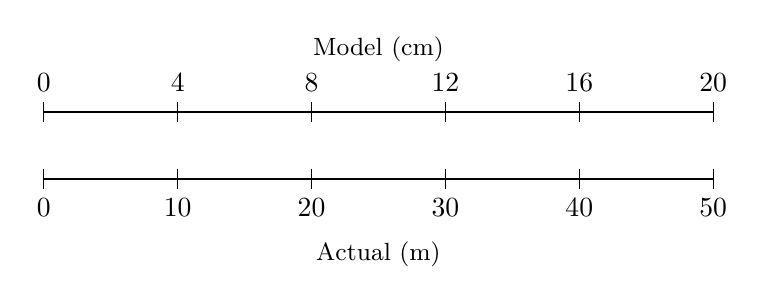
\begin{tikzpicture}[scale=0.85]
  \draw[thick] (0,0.5) -- (10,0.5);
  \draw[thick] (0,-0.5) -- (10,-0.5);
  \foreach \x/\lab in {0/0, 2/4, 4/8, 6/12, 8/16, 10/20}
    \draw (\x,0.35) -- (\x,0.65) node[above]{$\lab$};
  \node[above] at (5,1.1) {\small Model (cm)};
  \foreach \x/\lab in {0/0, 2/10, 4/20, 6/30, 8/40, 10/50}
    \draw (\x,-0.35) -- (\x,-0.65) node[below]{$\lab$};
  \node[below] at (5,-1.3) {\small Actual (m)};
\end{tikzpicture}
\end{center}

What actual length corresponds to a model length of $14$ cm?
\end{questionText}
\choiceA{$28$ m}
\choiceB{$35$ m}
\choiceC{$42$ m}
\choiceD{$70$ m}
\correctAnswer{B}
\explanation{From the double number line, the ratio is $\frac{10}{4} = 2.5$ m per cm. For $14$ cm: $14 \times 2.5 = 35$ m.}
\end{practiceQuestion}

\newpage
\section*{1-7-q25 \hfill \normalsize\texttt{tests\_questions\_bank\_2/topics\_additional/ch01-07-proportional-reasoning-with-scale-models.tex}}
\begin{practiceQuestion}{1-7-q25}{gsa}
\begin{questionText}
The scale drawing below shows the outline of a rectangular garden with a walkway across the middle.

\begin{center}
\begin{tikzpicture}[scale=0.8]
  \draw[thick,funGreen,fill=funGreen!10] (0,0) rectangle (6,4);
  \draw[thick,funOrange,fill=funOrange!20] (2.5,0) rectangle (3.5,4);
  \draw[<->,thick] (0,-0.5) -- (6,-0.5) node[midway,below]{\small $6$ cm};
  \draw[<->,thick] (-0.5,0) -- (-0.5,4) node[midway,left]{\small $4$ cm};
  \draw[<->,thick] (2.5,4.4) -- (3.5,4.4) node[midway,above]{\small $1$ cm};
  \node at (1.2,2) {\small Garden};
  \node[rotate=90] at (3,2) {\small Walk};
  \node at (0,-1.3) {};
  \node at (3,-1.3) {\small Scale: $1$ cm $= 3$ m};
\end{tikzpicture}
\end{center}

What is the actual area of the walkway in square meters?
\end{questionText}
\correctAnswer{$36$ sq m}
\explanation{Walkway on drawing: $1$ cm wide $\times$ $4$ cm long. Actual: width $= 1 \times 3 = 3$ m, length $= 4 \times 3 = 12$ m. Area $= 3 \times 12 = 36$ square meters.}
\end{practiceQuestion}

\newpage
\section*{1-7-q26 \hfill \normalsize\texttt{tests\_questions\_bank\_2/topics\_additional/ch01-07-proportional-reasoning-with-scale-models.tex}}
\begin{practiceQuestion}{1-7-q26}{gsa}
\begin{questionText}
The graph below shows the proportional relationship between model dimensions (cm) and actual dimensions (m) for a scale model.

\begin{center}
\begin{tikzpicture}[scale=0.5]
  \draw[step=1,gray!20,thin] (0,0) grid (10,10);
  \draw[thick,->] (0,0) -- (10.5,0) node[right]{\small Model (cm)};
  \draw[thick,->] (0,0) -- (0,10.5) node[above]{\small Actual (m)};
  \foreach \x in {2,4,6,8,10} \draw (\x,0.1) -- (\x,-0.1) node[below]{\tiny \x};
  \foreach \y in {2,4,6,8,10} \draw (0.1,\y) -- (-0.1,\y) node[left]{\tiny \y};
  \draw[thick,funBlue] (0,0) -- (10,8);
  \fill[funBlue] (0,0) circle (3pt);
  \fill[funBlue] (5,4) circle (3pt);
  \fill[funBlue] (10,8) circle (3pt);
\end{tikzpicture}
\end{center}

Using the graph, find the actual dimension for a model measurement of $15$ cm.
\end{questionText}
\correctAnswer{$12$ m}
\explanation{From the point $(5, 4)$: $k = \frac{4}{5} = 0.8$ m per cm. For $15$ cm: $0.8 \times 15 = 12$ m.}
\end{practiceQuestion}

\end{document}